\subsection{Абсолютное схождение}

\textbf{Задачи:}

У нас есть некоторая техника, которой мы опять воспользуемся

\begin{enumerate}
    \item $\integral{0}{1}\cos(\cfrac{1}{\sqrt{x}-1})\cfrac{dx}{x^{\alpha}}$

    Алгоритм состоит в том, чтобы оценить какой-то косинус множеством и на этом множестве играться, после того, как привели в нормальный вид. Вставлю доску Баскова, дабы стало понятнее.

    \begin{center}
        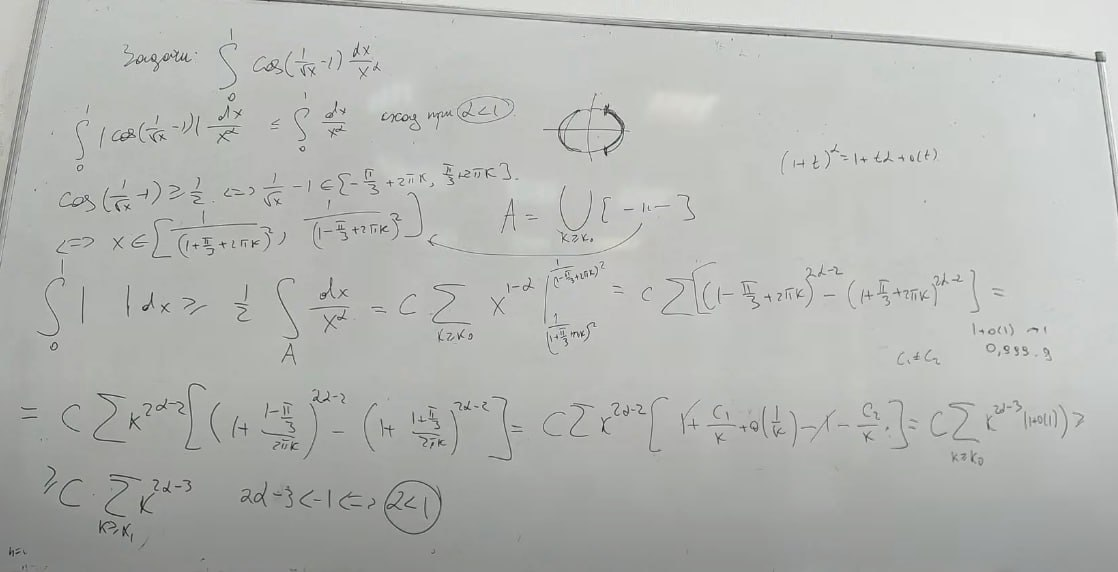
\includegraphics[width = 17cm]{assets/10_1.jpg}
    \end{center}



    Если $\alpha<1$, то интеграл сходится по верхним соображениям. Если $\alpha \geq 1$, то интеграл расходится по нижним соображениям.

    Чтобы понять условную сходимость пользуемся признаком дирихле (или абеля)

    Когда мы хотим  расходимость мы пользуемся третим концептом:

    \textbf{Критерий Коши о расходимости интеграла} (b точка разрыва):

    $\exists\varepsilon >0 : \forall \eta \in (a,b): \exists \eta_1, \eta_2 \in (\eta, b)$, такое что $|\integral{\eta_{1}}{\eta_{2}}f(x) dx| \geq \epsilon$

    В нашей задаче хотим:

    $|\integral{\eta_1}{\eta_2} \cos (\cfrac{1}{\sqrt{x}}-1)\cfrac{dx}{x^{\alpha}}|\geq \varepsilon$. Давайте возьмем тот же интервал, что и был:
    $$\left|\integral{}{} \cos (\cfrac{1}{x}) \cfrac{dx}{x^{\alpha}}  \right| \geq c k^{2\alpha -3}$$
    при $\alpha \geq \cfrac{3}{2}$ получаем, что она оценивается $c$ и показали существование.


    \item $\integral{0}{\frac{1}{2}}\left ( \cfrac{x}{1-x}\right)^{\alpha} \cos (\cfrac{1}{x^2})dx$

     \begin{center}
        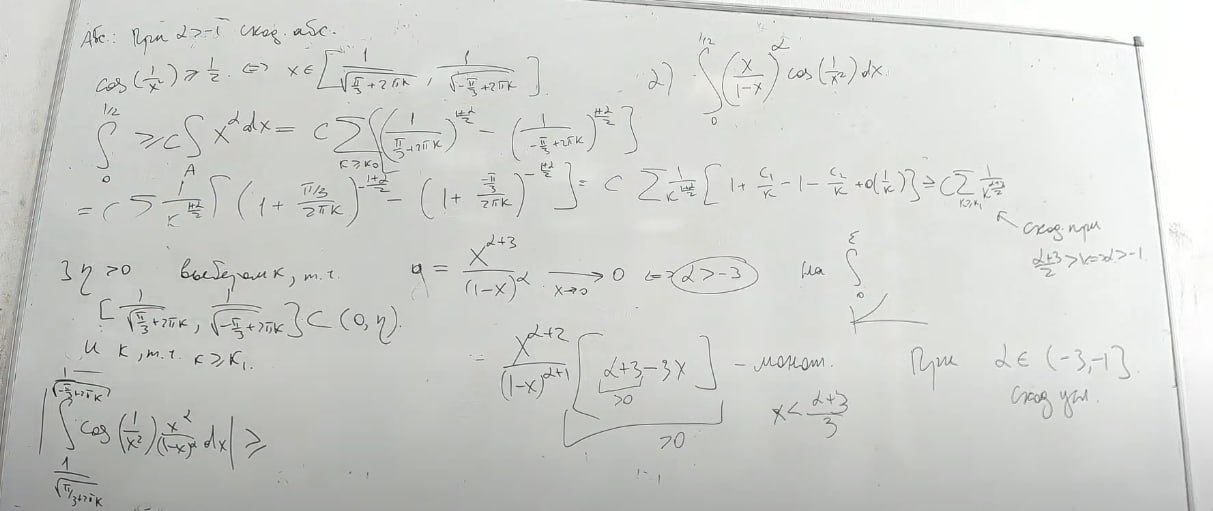
\includegraphics[width = 17cm]{assets/10_2.jpg}
    \end{center}

    И в концк мы оцениваем(то что снизу справа) $\geq c \cfrac{1}{k^{\alpha/2+3/2}}$
    
\end{enumerate}